% Question to answers during the next chapters
%%% Instruments used, set-up, materials
%%Description of the instruments and materials
%%How the instruments are set-up and what auxiliary connections might need to be used.
%%% add statment
\chapter{Algorithm to Optimize the Sailing Path for Laser Classes.} \label{sec:AlgOptSail}
%Introduction
The optimization problem for the minimal path is a problem frequently related with logistics and operations research. This type of problem is usually related with the \textit{Euclidean} shortest path and solved either with networking optimization or dynamic programming (\textit{\acrshort{dp}}). Although for Olympic sailing classes the optimal path is not related with distance but with time instead. \par \noindent 
Because of this, the research of this type of problem on sports is limited and it is mainly focused on yacht competitions. Whereas the laser class is the smallest and one of the most used sailboats on Olympic Classes. The objective of this section is not only to explain widely used methods but their elements and how they should apply to develop and algorithm for the Laser Olympic class.\par

Many techniques used on \acrshort{dp} and networking optimization can be used in combination with the \acrshort{vmg} criterion to developed and optimization algorithm for laser races.  Because the target's location and the geometrical domain are the features that allows the used of both criteria thus the optimal solution is found inside the polygon \cite{mitchell2000geometric}.\par 

The first part of this chapter explains how chapter \ref{ch:physics_sailboat} and chapter \ref{ch:weatherModel} are integrated to develop the algorithm to optimized the path of laser boats and obtain a minimal time path. But because most of the formulas on section \ref{sec:equil_equat} are generic, the adjustments required to describe the laser class are explained in the second part of this chapter. Followed by the explanation about the algorithm, details such as the objective function, the constraints and its validation. The validation of the algorithm is at the end of the chapter, and it provides information about the parameters defined by the user and at the initialization of the algorithm. \par 

%\section{Incorporation of the Wind Model into a Path Algorithm}
\section{Weather Routing Models and Path Algorithms for Sailboats}\label{sec:weatherRoute}

Uncertainty weather is a typical condition that not only yacht competitions have to manage but also maritime transportation. The direction-dependency of the vessel's velocity is seen as a series of regions where the flow's velocity is designed as uniform. This is characterizes as an anisotropic medium condition, and path algorithm problems with this characteristic has been solved with different methods \cite{dolinskaya2013fastest}. \par 
\noindent 
The most used methods related with vessels or yachts and anisotropic medium come from operations research and logistics. For example, from operations research these methods are dynamic programming (\acrshort{dp}), direct and indirect methods while the networking method is related with logistics. \cite{kelly2015transcription},\cite{mitchell2000geometric}. In the networking method the order in which the locations can be reach is not as important than time. \par 
The formulation of the problem is focus on the time and not in the length of the trajectory. However, it is the velocity of the sailboat the one that determines the direction of the sailboat and considers the wind properties. Because of this, equation \ref{eq:rabaudmintime} defines the time of the path to displace a sailboat between 2 points \cite{rabaudoptimal}. This is the easiest formulation of the problem but it shows how this problem differs from the shortest path approach.  \par

\begin{equation} \label{eq:rabaudmintime}
\begin{aligned}
T_{AB}=\int_{A}^{B} dt=\int_{A}^{B} \frac{dl}{v}  \\
\end{aligned}
\end{equation}

\subsection{Dynamic Programming and direction-dependence for Path Algorithms} \label{sec:dynProg}

\acrshort{dp} is a widely used technique to solve the optimal path problem for yachts and maritime transportation. The reason is because it breaks the main problem into multiple stages all connected. In this case, to move from point \textit{A} to point \textit{B} the trajectory is conformed for more than two points. Meaning that the main trajectory is conformed by multiple stages or smaller trajectories continuously coupled until it arrives to its final destination. \par \noindent 
The fact that one stage depends on the previous one, allows the recognition of the state of the variables implicated in that solution. This set of state variables is used to optimize the trajectory by iterating each stage until the optimal solution by stage is found. Thus the next stage always start from the optimal solution given by the last stage \cite{philpott2001optimising}. \par

In yacht competitions and maritime transportation, the trajectory is not only defined by the location of the points but also by the area within they are located. This area has to be defined first and later discretized not only to use variables that depends on its location and time, like wind and current, but also to apply \acrshort{dp}. The discretized area is composed by nodes and the line that connects 2 nodes is defined as an arc ($c_{arc}$). For example, node \textit{i} and \textit{j} is connected by the $c_{arc}(\textit{i,j,t(i)})$ which also depends on time (\textit{t}). Since the time at the starting point(\textit{$t_{A}$}) and the wind (\textbf{w}\textit{(i,j,t)}) and current(\textbf{c}\textit{(i,j,t)})  characteristics are known, the minimal time path using \acrshort{dp} is defined in equation \ref{eq:DP_minTimeP_Allsop}  \cite{zyczkowski2017method},\cite{allsopp2000optimal}.

\begin{equation} \label{eq:DP_minTimeP_Allsop}
f^*(i,t)=
\begin{cases}
0,  &  \\
\\
\noindent 
\displaystyle
\min_{j \in \Gamma_{i}} \Bigg[c_{arc}(i,j,t)+f^*\Big(j,t + c_{arc}(i,j,t)\Big) \Bigg]\\
\end{cases}
\end{equation}
\hspace{20mm} otherwise
\begin{equation}
j^*(i,t)=
\noindent 
\displaystyle
arg \min_{j \in \Gamma_{i}} \Bigg[ c_{arc}(i,j,t)+f^*\Big(j,t + c_{arc}(i,j,t)\Big) \Bigg], \quad i \neq n_{finish} 
\end{equation}

The equation explains how the time is minimized at each node until the final destination,point \textit{B}, is reached. $f^*$\textit{(i,t)} is the time at node (\textit{i,t}) which is optimal time resulting from the previous stages. $j^*$\textit{(i,t)} is the next node from \textit{i} on the optimal path, while $\Gamma_{i}$ is the set of subsequent nodes of \textit{i}. The minimal time of equation \ref{eq:DP_minTimeP_Allsop} to move from node \textit{i} at time \textit{t} when the next node is \textit{j} is given by:\par 
\begin{equation*}
    c_{arc}(i,j,t)+f^*\Big(j,t + c_{arc}(i,j,t)\Big) 
\end{equation*}

\noindent
Figure \ref{fig:dp_Allsop} is the graphical explanation of the equation to determine the minimal time from node 1 to 5, starting at time 1 (\textit{n(1,1)}). Node 5 ($n_{5}$) can be reach by 3 different paths, or in other words, there are 3 alternative nodes before $n_{5}$ can be reach.  The nodes 2, 3 and 4 can be reach at different times, the minimum time between them is given by $n_{4}$ with a time of 2 (\textit{n(4,2)}). The next arc is formed from $n_{4}$ to $n_{5}$ and because the starting time of $n_{4}$ is the minimal/optimal time for the first stage, the final time is then the minimum time path from $n_{1}$ to $n_{5}$. \par \noindent
These state-space algorithm for the shortest path includes explicitly the time dimension \cite{allsopp1998stochastic}.

\begin{figure}[hbt!]
    \centering
    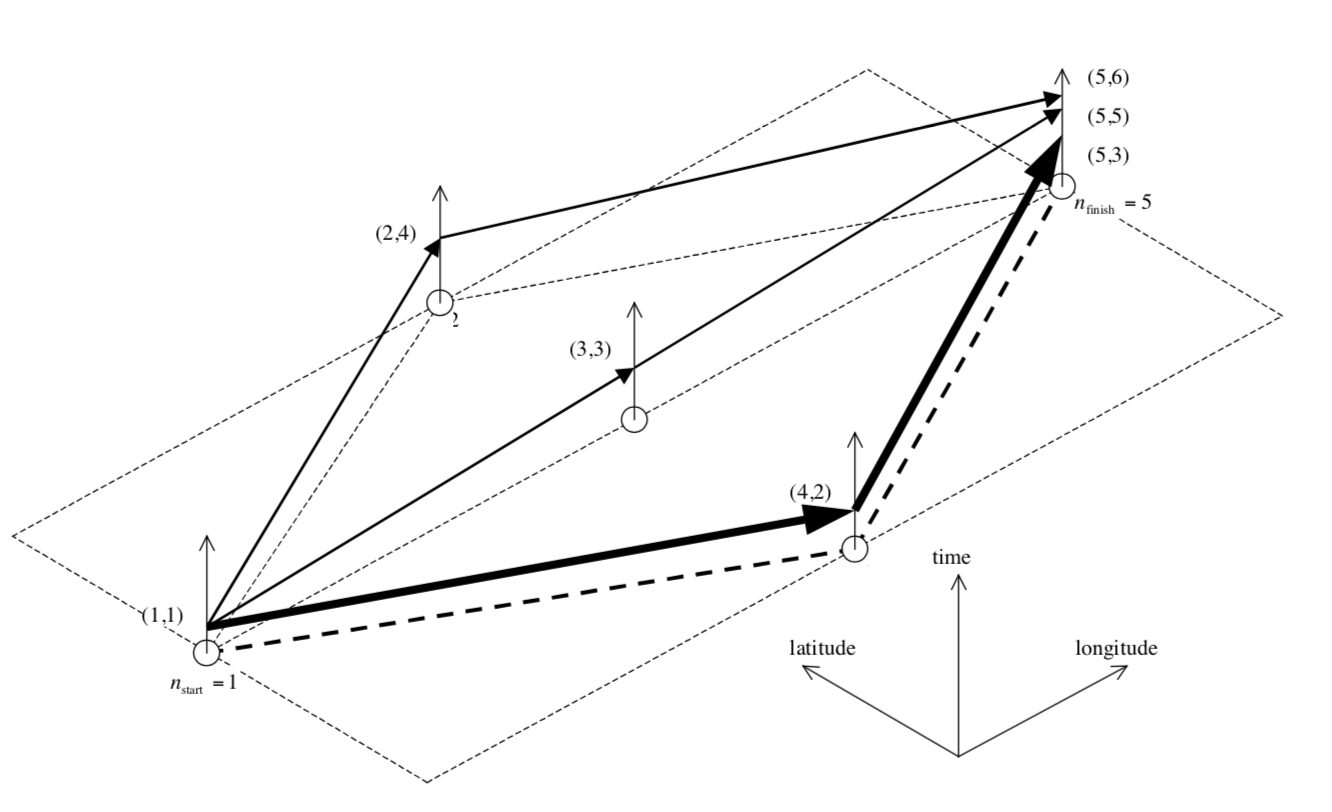
\includegraphics[width=.85 \linewidth ]{Allsopp1.png}
    \caption{Minimal Time Path from node 1 at time 1 (\textit{n(i,t)=n(1,1)}) to node 5 using \acrshort{dp}. The minimal time path to move from node 1 to 5 has go through node 4 and the path is indicated by the thicker  line \cite{allsopp2000optimal}.}
    \label{fig:dp_Allsop}
\end{figure}
\par 

An alternative process to discretize the area is based on the grid method and the heading decision, which is driven by the maximum velocity of the sailboat. This method can be related with the \acrshort{vmg} criterion because the same distance from the starting point can be reached at different times. Here, the heading-angle decision is discretized by intervals of size $\Delta \Psi$, clockwise and counterclockwise as a result multiple sub-routes are generated. If the symmetry of the \acrshort{vpp} is taken into account, some nodes and sub-routes can be represented within a diamond shape \cite{xing2012path} \cite{zyczkowski2017method}. \par \noindent
The number of stages($n_{stages}$) along the straight sailing distance (\textit{L}) between point $P_{0}$ and $P_{n}$ determines the shortest distance between (\textit{L} $\backslash n_{stages}$ ). In this case $n_{stages}$ can have any value bigger than 1 and it can be seen as the number of attacks that the seamanship could perform. The bigger the number the longer the time of the computational effort to determine the trajectory of the optimal time path \cite{xing2012path}. \par 
\noindent
The optimal heading is finding when the next stage is reached at the minimal time. In this case it is possible that multiple nodes arrive at the same time to the next stage. For this reason, the sub-routes have to been stored and the process continues until the destination point is reached. The algorithm to estimate the minimal time path is similar to the $c_{arc}$ process, the difference is in the from in which the area and stages is determined. The heading-direction approach sometimes uses additional factors over directions where the speed is the maximum. \par

Figure \ref{fig:diamondshape_subR} shows how the heading decision works. In this particular case, e all the sub-routes from $P_{0}$ to $P_{n}$ are contained into a diamond shape. Each node is describe by the stage and the node-number per stage, $P n_{stage},i_{sub-route}$ which is determined by the size of $\Delta \Psi$. The nodes over the edges of can only reach the half of nodes compared with the nodes at the center. The number of clear stages represented here are 6 and on each node there a maximum number of sub-routes is 21 and a minimum of 10. It is importance to remember here the concept of the \textit{no-go-zone} from section \ref{sec:VPP} because it could reduce the range of the heading direction angle.\par 

%\begin{figure}[hbt!]
%\centering
%  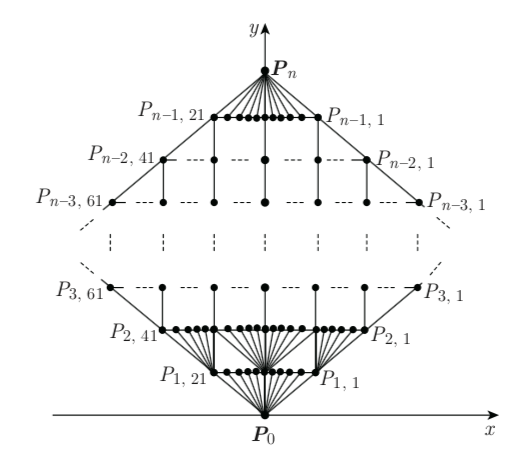
\includegraphics[width=0.6\linewidth]{legyachtxing.png}
% \caption{Leg yatching model \cite{xing2012path} }
%\label{fig:xing_nodesi}
%\end{figure}

\begin{figure} [hbt!]
  \centering
  \subfloat[Sailing Area Discretization for a Sailing Path from point A to B \cite{zyczkowski2017method}.]
  {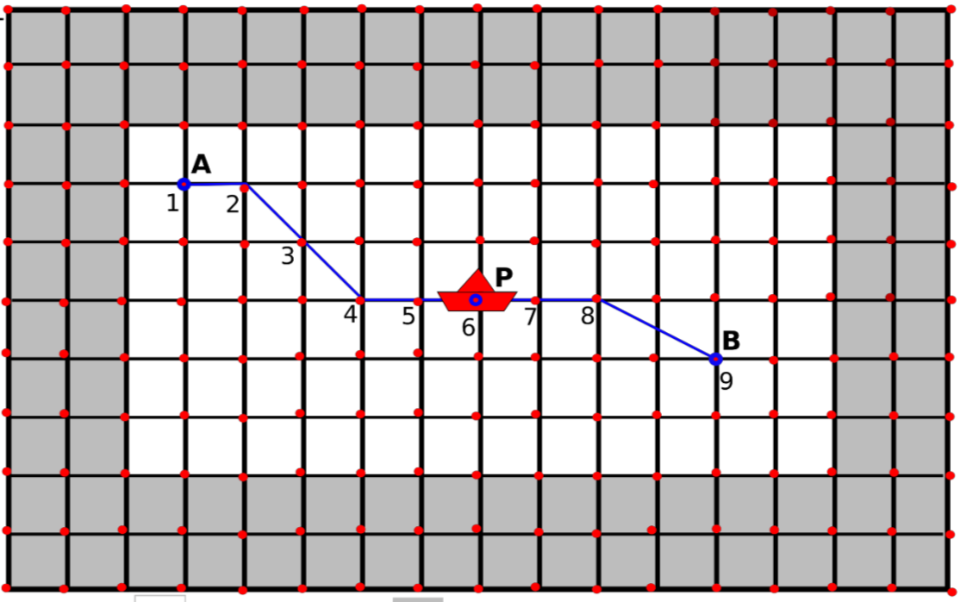
\includegraphics[width=0.33 \linewidth]
  {Sailing_area_heading.png}\label{fig:GridAreaSail}}
  \hfill 
  \subfloat[Heading Directions at a node, 8 angle discretizations \cite{zyczkowski2017method}.]{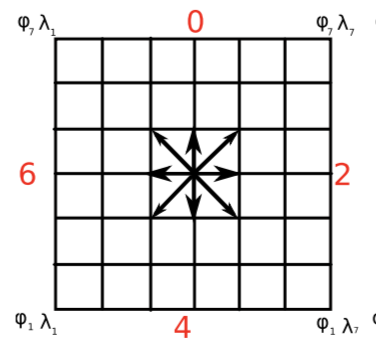
\includegraphics[width=0.22\hsize]
  {HeadDirNode.png} \label{fig:HeadAngle_Discret}}
  \hfill
  \subfloat[Diamond Shape with the Sub-routes for a heading-angle discretization to move from $P_{0}$ to $P_{n}$ \cite{xing2012path}.]
  {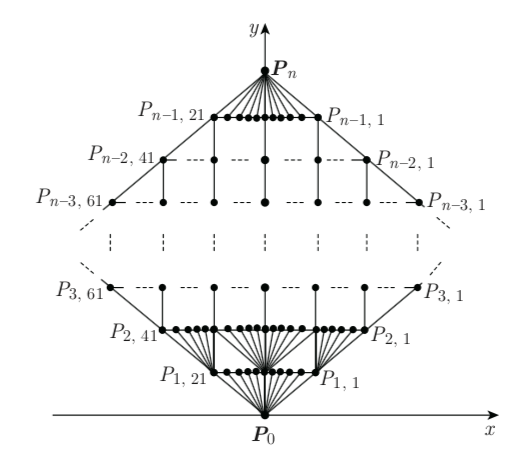
\includegraphics[width=0.33 \linewidth]{legyachtxing.png}
  \label{fig:diamondshape_subR}}
  \caption{Area discretized with a sailing path and Heading Angle discretization}
\label{fig:AreaDiscret} 
\end{figure}

\subsection{Path Algorithm Using Isochrones} \label{sec:isochrones}
A common solution with visual information obtained with \acrshort{dp} in weather routing are the isochrones. The isochrones lines compose a map where each line shows the maximum distance a sailboat can reach during a certain time. Moreover, this map can be seen as the visual representation of the \acrshort{vpp} over different anisotropic media when the weather variation is minimal \cite{allsopp1998stochastic}. \par 
A similar approach relates this type of solution with geometrical optics more specific with wavefronts. This analogy is because the speed of the wavefront depends on the refractive index of the material \cite{rabaudoptimal}.Figure \ref{fig:isochrone_ex} shows how the \textit{qtVlm} software uses isochrones to determine the optimal path for a generic yacht.\par

\begin{figure}[hbt!]
    \centering
    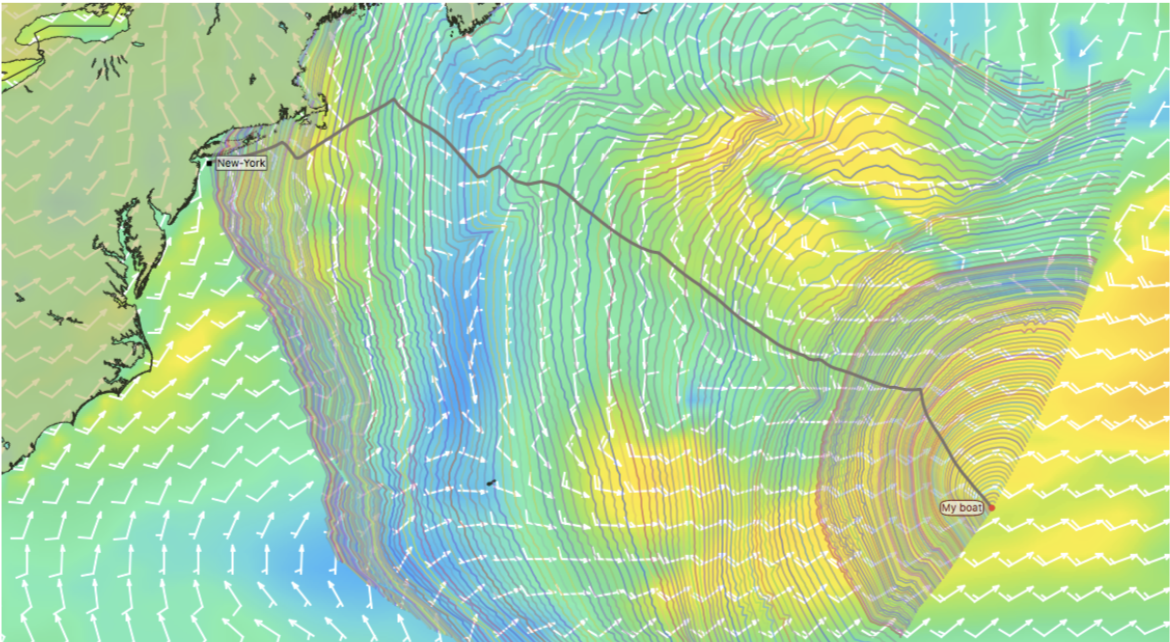
\includegraphics[width=.75 \linewidth]{isochrone_ex.png}
    \caption{Optimal Path Solution from qtVLm software using isochrones for a generic Yacht from a random location over the Atlantic to New York. The optimal path is the gray thick line, the wind direction is indicate by the white arrows.. The \cite{rabaudoptimal}. }
    \label{fig:isochrone_ex}
\end{figure}

The visual information presented by most these algorithms has been employed by various weather routing software. Despite of this, the use of them in sports and in Olympic Sailing Classes is limited. This because they are designed for long-distance yachts races or for maritime-logistics purposes. In both cases, the weather model is assumed to be homogeneous in space and time and frequently loaded from public sources. Meaning that the time step and grid size is much bigger than the required for Olympic Sailing races. Furthermore, when it is used for maritime-logistics purposes the vessels are equipped with communication and other measured systems that accounts for weather variations. \par
Despite the advantages of the isochrones techniques and its usage on large course races, the number of application for short courses is limited. The reason is because the weather is assumed to be perfectly known and even when the \acrshort{vpp} is assumed symmetric the algorithm doesn't explain or shows the limitations of choosing the symmetric path not even as an alternative for some space-time-intervals.\par    

%The envelop shape of the VPP used in \cite{rabaudoptimal} was explained in detail by \cite{dolinskaya2009optimal}.This type of shapes represent a feasible region where a vessel can moves in a straight line in a period of time from the origin; and it was called     \textit{linear path attainable region} for point (0,0)" \cite{rabaudoptimal}.
% resumen 
% points to include use of stages to set the path
% the discretiation of the area, and the wind is assumend location is know
% weather is perfectly know
% alssop interpolation 
% include advantages
\hspace{5mm}
In resume,
%As explained at the beginning of this section
\acrshort{dp} is a flexible method used to find the optimal sailing path and widely used for weather routing. The main characteristics of the previous techniques that have be considered for the development of the laser path algorithm are explained afterward. Before starting any sailing path, first it is important to define the area within any path might take place. This is not only because of the wind or current model but because inside that area a set of stages have also to be defined. This area for the sailing path have to cover effectively all the alternatives so the minimal time path can be found. \par 
After the area is defined it has to be discretized, the grid approach is commonly used. By using the grid it is easy to locate the node for either the node or the arc and to find the value for both wind and current. The discretization is directed related with the granularity of the problem and at the same time with the computational effort. \par 
The next characteristics to define is the number of stages is a free number that must be taken with care. The number of stages in combination with the number of variables define the state-space vector. This vector has to been estimated and later on compared as many arcs or nodes were determined. As a consequence of the size of the vector the computational effort can be affected and at this point the number of operations could grow exponentially.

\section{Adapting the Yacht Model to the Laser Class} \label{sec:laser_yacht}

Most of the research either for path planning or for the physic model for sailboats are related with yacht or with bigger boats such as sailing vessels. Figure shows the differences on heights for the mast only, where a the AC45 yacht race has a height of 25.5 m while the Laser Olympic class mast's height is 6.1 m. Equations on section  \ref{sec:eq_of_motion} are generic an applicable to any kind of sailboat. Hence to represent properly the laser class some modifications have to made before to properly represent its motion.\par 
\begin{figure} [hbt!]
    \centering
    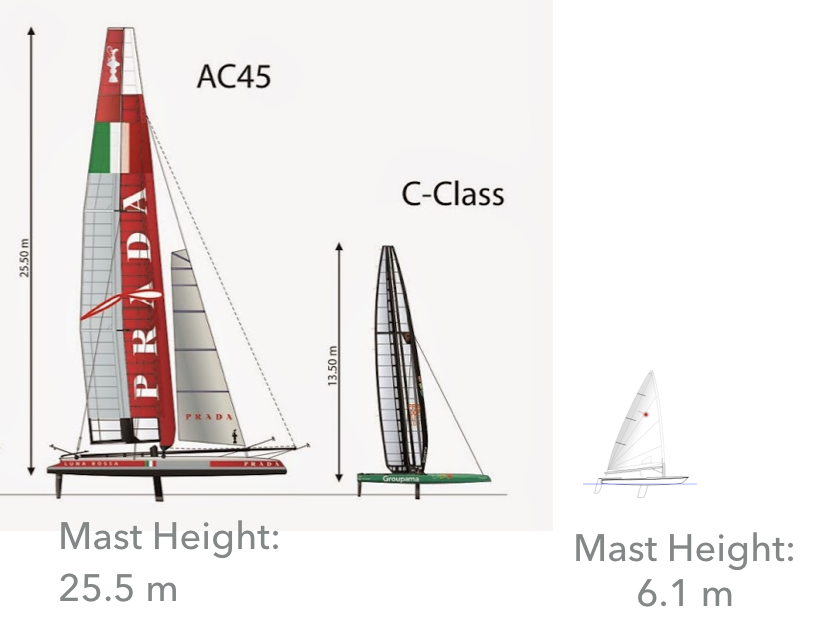
\includegraphics[width=0.75 \linewidth]{yacht_comp.png}
    \caption{Mast Height Comparison between two yachts models AC45 and C-Class versus the Laser Olympic Class, side view. \cite{yacht_compw}.}
    \label{fig:yacht_mast_height}
\end{figure}
The sailboat of the laser class is the dinghy one of the smallest boats propelled by wind, with a maximum weight of 59 kg \cite{sailoly}. Therefore its balance on the \textit{heave axis} (\acrshort{heave_ax}), between the heel angle (\acrshort{heel_ang}) and righting moment (\acrshort{right_m}) is determined by the ability of the crew to adjust its posture over each side of the boat. The posture of the crew respect to the boat is determined by the wind speed and direction mainly. So it can be said that the crew's posture is a response to the weather variations \cite{marchajaereo1979}.\par 

Even when these assumptions are implicit to keep the sailboat analyses in 2-dimensions and developed the \acrshort{vpp} there's is being some discussion about it \cite{philpott1993yacht},\cite{larsonprinciples}. The discussion are related not only with the posture but also with the impact of crew's mass (\acrshort{crew_m}). Since for Olympics Sailing Races it could represent more than $50 \% $ of the total mass of the sailboat (\acrshort{m})\cite{day2017performance}. These without considering the rate of change of these postures adjustments and the assumption that its centroid (\acrshort{crew_m}) is located in the center of gravity (\acrshort{c_g}) of the sailboat. \par 

A deeper analysis and comparison between the adaptations on the standard \acrshort{vpp} were addressed about the coefficients and forces related with the sails. The comparison of the different coefficients values include the data taken from the Offshore Rating Congress (2013) and the observations made in other works \cite{day2017performance}, \cite{carrico17symp}, \cite{binns2002development}, \cite{flay1996twisted}. Furthermore, these modifications correspond to the addition of the \textit{reef} and \textit{flat} coefficients of the sail. Particularly, they account for the fact that dinghy's sail do not reef against strong winds. As a consequence of this, the drag and lift coefficients must been adjusted during the upwind and downwind course \cite{carrico17symp}. \par \noindent
The adaptations directly related with the 
%were divided according the 
aerodynamic 
%and hydrodynamic 
forces, as a result of the \textit{flat}, \textit{twist} coefficients and the \textit{spill}(\acrshort{spill}) variable 
%were included. 
are showed next. These coefficients model the behavior of the sails and the athlete under strong wind conditions and it includes not only the upwind conditions but also the downwind course \cite{day2017performance}. % in additions to some conditions to be included when a downwind course is sailedIn \cite{day2017performance}. \par 
Therefore, equations \ref{eq:Cd} and \ref{eq:Ct} are modified to account the required adjustments. \par \noindent 
Then \acrshort{spill} modifies equation \ref{eq:Ct} and is shown in equation \ref{eq:liftMod} where \acrshort{Ctwist} has a value of  \textit{8.0} and \acrshort{twist} which is the \textit{twist variable} has a range value of [0,1], \acrshort{CDv} and \acrshort{CLmax} is obtained by interpolation from tabulated values and it depends on \acrshort{b_aw} while \acrshort{CDs} has a value of \textit{0.005} and \acrshort{ARE} is based on the rig geometry and calculated according it \cite{day2017performance}. \par \noindent  
Equation \ref{eq:Cd} is replaced by \ref{eq:draftMod}, the values taken were the smallest with an reduction of the area of 20 \% to consider shielding from the cockpit \cite{day2017performance}.\par 
%The effective aspect ratio ARE is calculated from the geometric aspect ratio based on rig geometry

\begin{equation} \label{eq:liftMod}
    C_{t}^*=C_{Dv}(\beta_{aw}-s)+C_{Dp}+f^2 \cdot C_{Lmax}^2 \cdot (\beta_{aw}-s) \cdot \Big(\frac{1+C_{twist} \cdot t^2}{\pi AR_{E}} + C_{Ds}\Big)
\end{equation}

\begin{subequations} \label{eq:draftMod}
 \begin{align}
  C_{d}^*= 1.075 && \text{for the frontal area} \label{eq:FrontalAreaDraft} \\
  C_{d}^*= 0.954 && \text{for sideways area} \label{eq:SideAreaDraft}
 \end{align}
\end{subequations}

\par 
The literature regarding \acrshort{vpp} for laser boat classes is limited and it is mainly accounted in \cite{day2017performance}, the comparisons made here are only valid for wind speed between  4 and 16 knots, while races are performed up to 25 knots. This range have to be consider in the developed of the algorithm to find the optimal path since it is the velocity of the wind that determines the direction that should be taken in order to maximize the \acrshort{vmg} criterion. \par 

\section{The Optimization Algorithm for the Minimal Time Path}
At this point, all the elements required to define the algorithm for the sailing path have been described. In this section those elements are going to be implemented in a similar order in which they were described. First the parameters of the Laser are going to be described so its \acrshort{vpp} can be estimated, then the area for the sailing race has to be defined and finally how the optimization was setting up and validated. 

\subsection{The Laser Olympic Class}
As mentioned before the Laser sailboat is the smallest class of the Olympics Sailing Classes and it is shown in figure . The dimensions and parameters that describe the laser are regulated by the \acrfull{ilca} and they are showed next in addition to some coefficients previously defined. Figure shows a side view of the Laser Standard and Laser Radial which are Olympic Classes. %For the \acrshort{Asail} and \acrshort{Asail_La} equation is used, where $L_{luff}$ refers to the luff lenght and $L_{foot}$ is the length of the foot, for which the maximum dimensions were used.
%\begin{equation} \label{eq:sail_area}
 %   A_{sail}=0.5 \cdot L_{luff} \cdot L_{foot}
%\end{equation}
\begin{description}
        \item \acrshort{mboat}= 59 [kg] \acrlong{mboat}
        \item \acrshort{Loa} = 4.2 [m] \acrlong{Loa}
        \item Beam = 1.37 [m] Beam width
        \item \acrshort{Tc} = 0.787 [m] \acrlong{Tc}
        \item \acrshort{Asail_La} = 5.76 [$m^2$] \acrlong{Asail_La}
        \item \acrshort{Asail} =  7.06 [$m^2$] \acrlong{Asail}
        \item \acrshort{Ak} = 0.23 [$m^2$] \acrlong{Ak}
        \item \acrshort{Ar} = 0.11 [$m^2$] \acrlong{Ar}
        \item \acrshort{Cdhull} = 0.02 [-] \acrlong{Cdhull}
    \end{description}
\begin{figure} [hbt!]
    \centering
    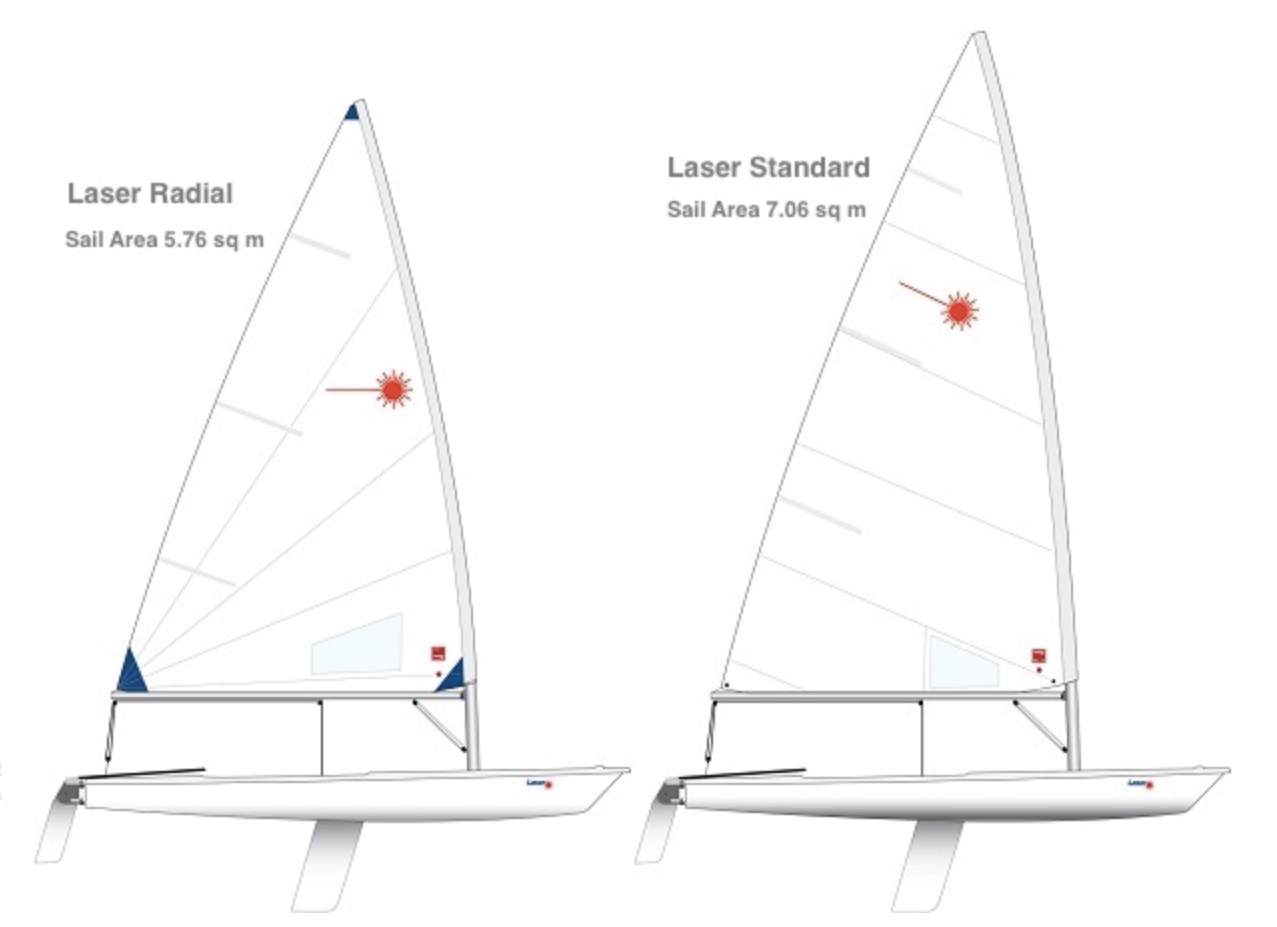
\includegraphics[width=0.64 \linewidth]{LaserOlympicClasses.png}
    \caption{Laser Olympic Classes. Laser standard refers to men category while Laser Radial is for women. The difference between them is only the size of the sail. \cite{2015LaserAssociation}}
    \label{fig:LaserSideView}
\end{figure}
The equations of section \ref{sec:eq_of_motion}, uses the added mass over each axis which according \cite{keuning2004mathematical} can be determined by equations \ref{eq:mx_add} and \ref{eq:my_add}. At this point the \acrshort{crew_m} is required and for the purposes of this research the maximum value suggested by \cite{laser_opt} is used. 
\begin{equation}\label{eq:mx_add}
    m_{x}=2\frac{T_{c}} {Loa} m_{T}=2\frac{T_{c}} {Loa} (m_{boat} + m_{c})=2\frac{0.787}{4.2}(59+70)=48.34 \text{ kg}
\end{equation}
\begin{equation} \label{eq:my_add}
    m_{y}=0.25 \cdot m_{T}=0.25 \cdot (59+70) = 32.25 \text{ kg}
\end{equation}

Most of the coefficients used on the equations of section \ref{sec:eq_of_motion} can be found on tables, however they can be approximate by using sine and cosine functions \cite{rein2012tra},\cite{moreira2011guidance}. These coefficient approximations are referred to the keel ($C_{i,keel}$) and rudder ($C_{i,rudde}$) only and they are shown next, the sub-index \textit{L} is for the \textit{lift} while \textit{D} is for the \textit{drag}. \par 
\begin{subequations} \label{eq:keel_coeff}
    \begin{align}
        C_{L,keel}=0.615sin(2\beta_{k_{a}})+0.025 \label{eq:keel_Liftcoeff}\\ 
        C_{D,keel}=-0.55cos(2\beta_{k_{a}})+0.55 \label{eq:keel_Dragcoeff}
    \end{align}
\end{subequations}
\begin{subequations} \label{eq:rudder_coeff}
    \begin{align}
        C_{L,rudder}=0.6175sin(2\beta_{r_{a}})+0.0325 \label{eq:rudder_Liftcoeff}\\ 
        C_{D,rudder}=-0.55cos(2\beta_{r_{a}})+0.55 \label{eq:rudder_Dragcoeff}
    \end{align}
\end{subequations}
Due to these approximations equations \ref{eq:Side_force}, \ref{eq:att_r} and \ref{eq:att_k} are modified and facilitate the separation of the \textit{lift} and \textit{drag} forces to use them. The angle of attack (\acrshort{a_a})is related with the \acrshort{b_aw}, therefore it is related with the trim angle of the sail (\acrshort{trim_sail}). The keel is a fix element and it is assumed rigid then its \acrshort{b_k_a} is the same as the \acrshort{b_ac}.   \par \noindent %The approximations related to the sail will not be used since equations \ref{eq:draftMod} and \ref{eq:liftMod} 
\begin{equation} \label{eq:app_current_ang}
    \beta_{ac}=atan2\frac{v}{u}
\end{equation}
\begin{equation} \label{eq:app_current_vel}
    V_{ac}=\sqrt{u^2 + v^2}=V_{boat}
\end{equation}
\begin{equation} \label{eq:keel_lift}
    F_{L,keel}=\frac{1}{2} \cdot \rho_{w} V_{ac}^2 A_{keel}C_{L,keel}(\beta_{ac})
\end{equation}
\begin{equation} \label{eq:keel_drag}
    F_{D,keel}=\frac{1}{2} \cdot \rho_{w} V_{ac}^2 A_{keel}C_{D,keel}(\beta_{ac})
\end{equation}
\begin{equation} \label{eq:angle_attack_rudder}
    \beta_{r_{a}} = \beta_{ac} - \delta_{r}
\end{equation}
\begin{equation} \label{eq:rudder_lift}
    F_{L,rudder}=\frac{1}{2} \cdot \rho_{w} V_{ac}^2 A_{rudder}C_{L,rudder}(\beta_{r_{a}})
\end{equation}
\begin{equation} \label{eq:rudder_drag}
    F_{D,rudder}=\frac{1}{2} \cdot \rho_{w} V_{ac}^2 A_{rudder}C_{D,rudder}(\beta_{r_{a}})
\end{equation}
\begin{equation} \label{eq:angle_attack_sail}
    \alpha_{a} = \beta_{aw} - \delta_{sail}
\end{equation}
The motion of the sailboat is dominated by the wind and this research is focus on the effects of the wind. As a result, the $\beta_{i_{a}}$ of the rudder and keel are treated as one component and substituted by $\alpha_{a}$ \cite{rein2012tra}. The implication of this substitution has two effects, first on the \acrshort{Rhull} and second on the lateral force. The coefficient related with the \acrshort{Rhull} has to account for thus it has to increase to \textit{0.025}. \textbf{The lateral forces is assumed to be in equilibrium all the time as a result, the \acrshort{v} velocity known as drift speed is neglected} hence equation \ref{v_dot} is omitted from the equations of motion for the Laser Class \cite{rein2012tra}.\par  
Another modification is related with equation \ref{eq:u_dot} which has to be modify to replace the hydrodynamic derivative expression ($X_{V\psi}$) by a damping expression showed on equation \label{eq:u_dotLaser}. The damping expression is related with a constant value  (\textit{Cnst}) of 0.3 according to \cite{rein2012tra}. \par
\begin{equation} \label{eq:u_dotLaserM}
    \Dot{u}=\frac{X_{TOT}}{m+m_{x}}-Cnst \Dot{\psi}^2
\end{equation}
To recapitulate all the previous changes, the equations of motion that describes the motion for the Laser Olympic Class are: \par 
\begin{equation} \label{eq:X_uM}
    X_{U}=\frac{1}{2}\rho_{w}V_{boat}^2 \cdot C_{D,hull}=\frac{1}{2}\rho_{w} \cdot V_{ac}^2 \cdot 0.025 
\end{equation}
\begin{equation}\label{eq:X_sailM}
       X_{sail}=F_{L,s}sin\beta_{aw}-F_{D,s}cos\beta_{aw} 
\end{equation}
\begin{equation}\label{eq:Forces_M} 
     X_{current}=m\cdot V_{boat} \Dot{\psi}= m\cdot V_{tc}^b \cdot \Dot{\psi}
\end{equation}
\begin{equation}\label{eq:X_TOTM}
    X_{TOT}=X_{U}+X_{sail}+X_{current}
\end{equation}
where:
\begin{equation} \label{eq:SailLiftM}
    F_{L,s}=\frac{1}{2}\rho_{a}V_{aw}^2 \cdot A_{s} C_{t}^*
\end{equation}
\begin{equation} \label{eq:SailDragM}
    F_{D,s}=\frac{1}{2}\rho_{a}V_{aw}^2 \cdot A_{s} C_{d}^*
\end{equation}
Finally the equations that describe the motion are:\par
\begin{equation}\label{eq:x_dotM}
\Dot{x}=u \cdot cos\phi + u_{tw} + u_{tc}
\end{equation}
\begin{equation}\label{eq:y_dotM}
\Dot{y}=u \cdot sin\phi + v_{tw} + v_{tc}
\end{equation}
\begin{equation} \label{eq:u_dotLaserMR}
    \Dot{u}=\frac{X_{TOT}}{m+m_{x}}- 0.3 \Dot{\psi}^2
\end{equation}

These modified equations serves only for the laser Olympic class and with them the \acrshort{vpp} can be estimated. Even so, at some wind velocities  %the approximations of 
equation \ref{eq:liftMod} %and \ref{eq:keel_coeff}
could be less accurate, specially at \acrshort{v_tw} close to 20 kn and above it. Since equations \ref{eq:liftMod} and \ref{eq:draftMod} work fine when the \acrshort{v_tw} is close to 10 kn \cite{day2017performance}, which is at the lower range of the \acrshort{v_tw} range defined by \cite{laser_opt}. \par 

\subsection{ VPP for the Laser Olympic Class}
The optimization of the minimal time path as showed in equation \ref{eq:rabaudmintime} requires to determine first the velocity which in this case \acrshort{v_aw}($\psi$). \acrshort{v_aw}($\psi$) is related with the wind speed and direction and considering the computational effort and the fact that the wind model is space and time discretized. The \acrshort{vpp} can be estimated first since the wind speed range rule ([4,25]kn) conditions the laser races. To estimate the \acrshort{vpp} not only the \acrshort{b_tw} but also the \acrshort{v_boat} has to be discretized with small steps values. \par \noindent 
Using the previous equations and replaced in equations from \ref{eq:X_tot} to \ref{y_dot} the \acrshort{vpp} can be obtained using an optimization method. The systems of equations can be solve over the angle range of [0,180 \degree] using the built-in function of \textit{fmincon} from \acrshort{matlab}\cite{rein2012tra}. The problem is defined as maximization of the \acrshort{v_boat} which means that all the forces are in equilibrium. However, any  optimization problem has to be defined in terms of the minimum value so the problem is defined as:
\begin{align}
    \text{minimize:}\qquad & -u(u,\psi,\delta_{s},V_{tw})  \label{eq:max}\\
\text{subject to:} \qquad & X_{TOT}=0
%& \Dot{v}=0 \\
%& \Dot{\psi}=0
\end{align} \label{eq:opt_vpp2}
instead of: 
\begin{align}
    \text{maximize:}\qquad & u(u,\psi,\delta_{s},V_{tw})  \label{eq:max2}\\
\text{subject to:} \qquad & \Dot{u}=0 \\
%& \Dot{v}=0 \\
& \Dot{\psi}=0
\end{align} \label{eq:opt_vpp}
Equation \ref{eq:max} shows that \acrshort{u} is the boat's velocity and it depends on itself which means that the system is not linear. Moreover, its influence on \acrshort{b_tw}, \acrshort{v_aw} determines the sail's forces. The control variables this problem are $\Dot{\psi}$ and \acrshort{trim_sail}, this last could have a value over the range of [0,180 \degree] but it should not cancel $\Psi$, during motion.
\par
\begin{figure}[hbt!]
    \centering
    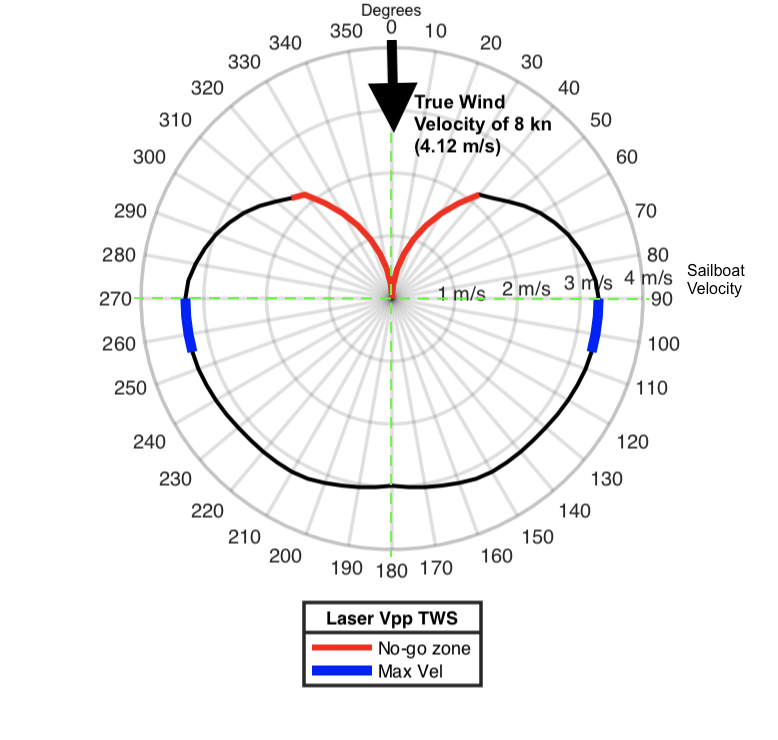
\includegraphics[width=.53 \linewidth]{Vpp_8.png}
    \caption{Full VPP for the Laser Class at 8 kn $V_{tw}$ coming at $0\degree$ from the North, the angles were discretized with and interval of $10\degree$} 
    \label{fig:Laser_Full_Vpp85}
\end{figure}
Figure \ref{fig:Laser_Full_Vpp85} shows the full \acrshort{vpp} of the Laser Olympic Class for a wind of 8 kn. In this graphic the direction of the wind is zero degrees from the North. The angle's interval is $10\degree$ and the \acrshort{v_boat} is indicated by the diameter of the circles in this case, it has a range value of [0,3.3] m$\backslash$s . In the figure the \textit{no-go-zone} is in the angle range of [0, 40] degrees and [320, 360] degrees while the maximum velocity of the boat can be reach in the angle range of [90, 115] degrees and [255, 270] degrees. \par 
\noindent
The \acrshort{v_boat} range taking out the \textit{no-go-zone} is [2,3.3] m$\backslash$s, the \acrshort{vpp} shape over the range of [90,270] degrees does no varies to much. The shape is close to a semi-circle, this means that under a downwind condition a straight trajectory could be more efficient if the tack loss time is bigger than the velocity change ratio while the \acrshort{v_tw} remains constant.  \par  

An alternative method to estimated the half of the  \acrshort{vpp} uses wind measurements for the speed and its direction. These measurements however does not have a constant interval, so to predict any other wind speed and its direction, the measured data is interpolated  
%Interpolating between known values can then give predicted maximum speeds for any true wind angle and true wind speed
\cite{philpott2001optimising},\cite{allsopp2000optimal}. For the purpose of this project, some wind measurements for wind speed  were provided by \acrlong{sailctr}. \par \noindent 
The interpolation used for the missing points was the \acrfull{pchip} from \acrshort{matlab}. The use of this data not only serves as validation for the \acrshort{vpp} calculations but also as data source. This because many of the research regarding \acrshort{vpp} for the Laser Olympic Class only cover a wind speed range of [9,12] kn \cite{day2017performance} and the measurements provided are out of this range and they are shown in figure \ref{fig:hvpp_MeasData}.\par \noindent
Figure \ref{fig:hvpp_MeasData} indicates the measurements taken with black asterisk, the rest of the points, therefore the line is the result of the \acrshort{pchip} interpolation. The wind measured are referred as \textit{TWS} and it is assumed to comes from the North, top of the graph. The \acrshort{vpp} is assumed to be symmetric and due to this, the measurements where only taken in the range of [0,180] degrees. \par 
\begin{figure} [hbt!]
    \centering
    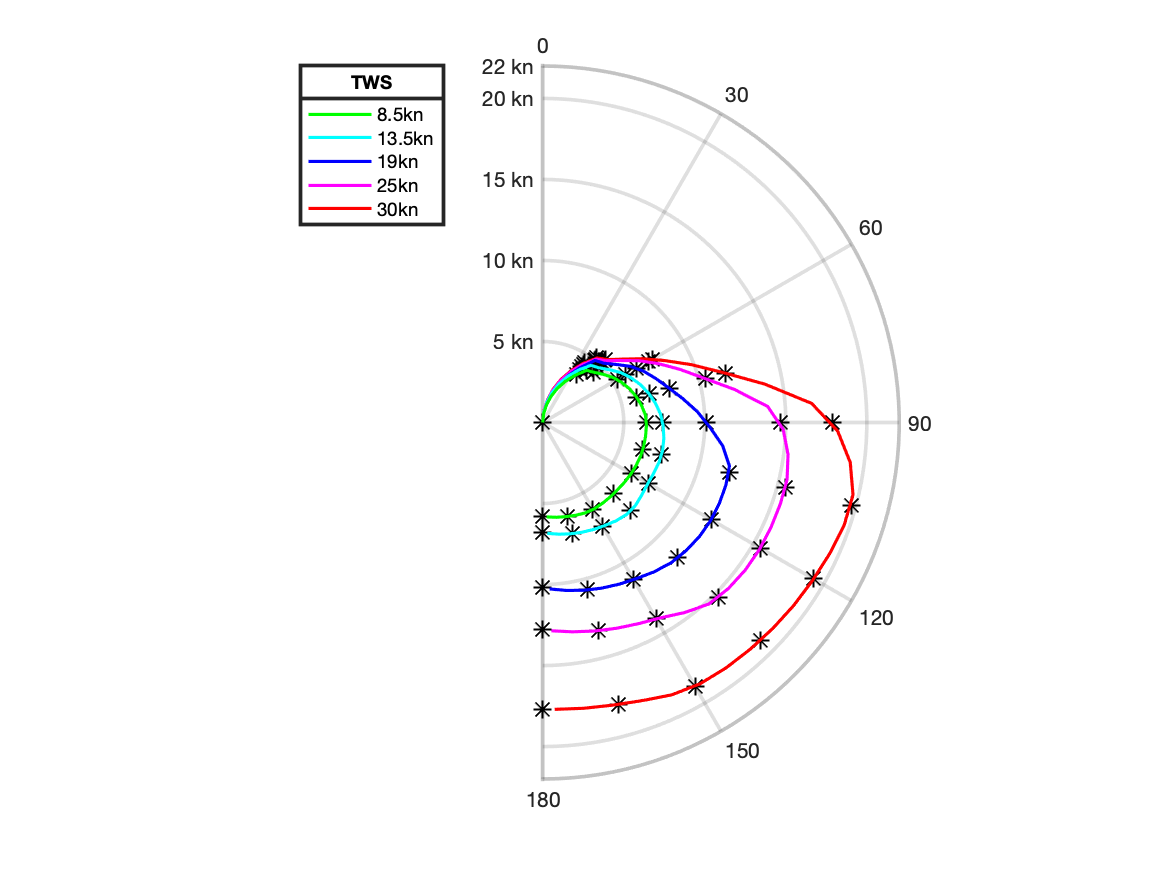
\includegraphics[width=0.72 \linewidth ]{Half_Vpp_laser2.png}
    \caption{Vpp developed with measurements provided by $InnoSportLab\textsuperscript {\textregistered}$, The Hague. The measurements are indicated with black asterisk. The results of the interpolation varies according the wind velocity (TWS)}
    \label{fig:hvpp_MeasData}
\end{figure}
The measured data not only serves to develop the \acrshort{vpp} but also to validate some of the assumptions previously made. Now that the\acrshort{vpp} was determined the formulation of the minimal time path for the Laser Sailing Class can be described.  \par 

\subsection{The Objective Function: The Minimal Time Path}
At this point all the elements required to develop the algorithm have been explained. In this section their implementation is going to take place. The objective is to find the path with the minimum time, regardless the type of sailing course. Figure \ref{fig:SailModes_Man}, shows the three types of courses with its main maneuvers and angle range is not especify for each condition since this range depends mainly on the \acrshort{vpp} and sailor preferences. For example under a downwind condition, even when shifts on direction can be made most of the sailor follows a straight line rather than a zig-zag trajectory. \par
\begin{figure} [hbt!]
  \centering
  \subfloat[The 3 main modes to sail respect to the wind direction.]
  {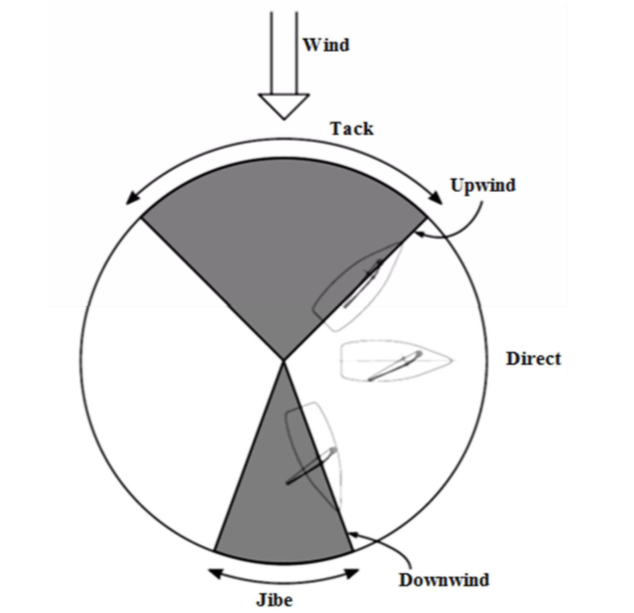
\includegraphics[width=0.45 \linewidth]
  {SailingModes.png}\label{fig:SailModes}}
  \hfill 
  \subfloat[Types of Maneuvers for sailing according the boat and wind direction .]{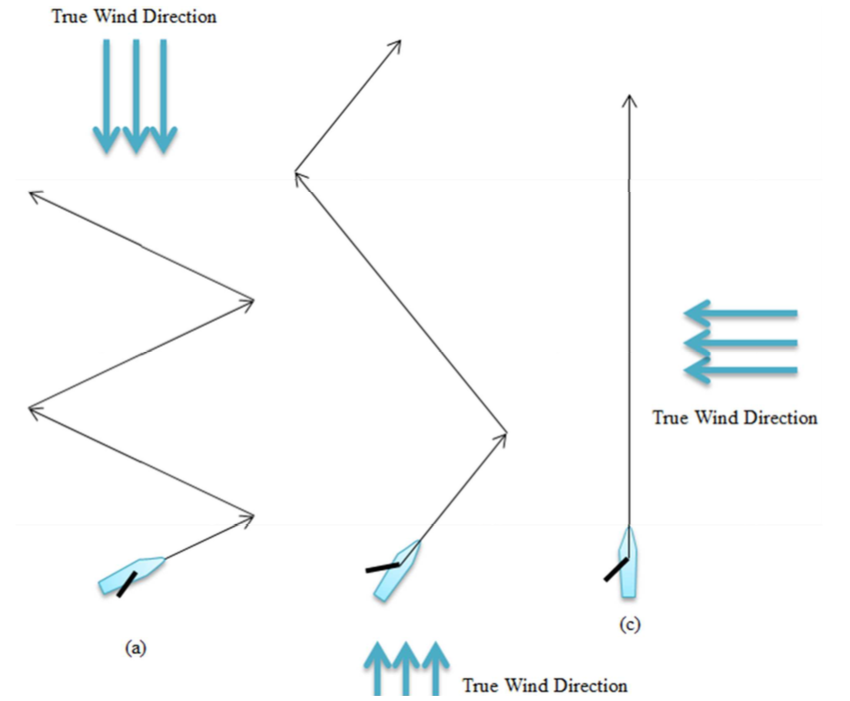
\includegraphics[width=0.45 \linewidth]
  {SailinMAnu.png} \label{fig:maneuversType}}
  \caption{Type of courses and its Maneuvers \cite{Alves2014ASailboat}}
\label{fig:SailModes_Man} 
\end{figure}

The combination of at least two of these sail-modes determines a race for Olympic Sailing Competitions. Each sail-mode over the course is defined as \textit{Leg}, them the minimal time for the race is given by the minimal time on each leg. The optimization problem that accounts for a set of leg is defined as a multi-phase problem because all the phases are connected. Hence the minimal time path for the Olympic Laser races is based on equation \ref{eq:rabaudmintime} and defined as: \par 
\begin{align}
%\min_{j \in \Gamma_{i}}\\ 
    \text{min } & T=
    %\int_{t_{0}}^{t_{f}} dt=
    Leg^{i}(\Psi_{k,n},t_{f_{k,n}})+ \int_{t_{0}}^{t_{f}} \frac{dl_{k,n}^i}{v_{k,n}} \quad ,k \in \{1,2,3\} \label{eq:minTO}\\
\text{subject to:} \quad & \Dot{x}=u(\Psi)cos(\Psi) + u_{tw}+u_{tc} \\
\quad & \Dot{y}=u(\Psi)sin(\Psi) + v_{tw}+v_{tc}
\end{align}
the boundary conditions are:\par
\begin{align}
   \quad & t_{0}^1=0 \label{eq:InitialTime} \\
   \quad & t_{0}^{i}= t_{f}^{i-1} \label{eq:FinalTimeLeg} \\
   \quad & x(0)^i=x_{1}\label{eq:locIniX} \\
   \quad & x(t_{f})^i=x_{2}\label{eq:locFinX} \\
    \quad & y(0)^i=y_{1}\label{eq:locIniY} \\
   \quad & y(t_{f})^i=y_{2}\label{eq:locFinY}
\end{align}
the state limits for the variables are:
\begin{align}
    \quad & x_{min}^{k,n}<x(t)^k<x_{max}^{k,n} \label{eq:xlox_leg_alt}\\
   \quad & y_{min}^{k,n}<y(t)^k<y_{max}^{k,n} \label{eq:ylox_leg_alt}\\
   \quad & \Psi_{min}<\Psi(t)< \Psi_{max} \label{eq:Dirlox_leg_alt}
\end{align}
The tack maneuver, which refers to the change in direction are pare of the constraints so they have to be defined also, as \par
\noindent
for the tack to port:
\begin{equation}\label{eq:tackportC}
70\degree < \Psi^{i,n_{max}-1}(t_{f}^{i}) -
\Psi^{(i+1),n_{i+1}}(t_{0}^{i}) < 110 \degree
\end{equation}
\noindent
and for the tack to starboard:
\begin{equation}\label{eq:tackstarbC}
-110\degree < \Psi^{i,n_{max}-1}(t_{f}^{i}) -
\Psi^{(i+1),n_{i+1}}(t_{0}^{i}) < -70 \degree
\end{equation}
To connect all the legs, not only the tack angle are defined but also its locations, as:
\begin{align}
    \quad & x^{i+1}(t_{0}^{i+1})=x^{i}(t_{f}^{i})\label{eq:x_linkC}\\
    \quad & y^{i+1}(t_{0}^{i+1})=y^{i}(t_{f}^{i}) \label{eq:y_linkC}
\end{align}
Because inside each leg numer of \textit{n} st
\subsection{Defining the Constraints for the Path Generation}
\subsection{Validation of the Algorithm}
\section{Considerations: Results from  the Validation}

%\subsection{Wind Model}
%Weather model forecast are calculated  by super computer and updated every three hour according regions. Different agencies have developed models to predict it in global terms. The local prediction are made based on it with via extrapolation and interpolation between local measurements with the intention to predict it every hour, for local purposes. The global and open information is stored in what is know as GRIB or NET files. This files, GRIB, is downloaded according the region of interest the common grid size provides is a 3 km square. 
%In \cite{binns2002development} the simulator use a guts wind model  with the next parameters: the time step was defined as 60 seconds and the length of 200 m. It can be said that the grid 

